\documentclass[12pt]{article}
\usepackage{amsmath}
\usepackage{enumitem}
\usepackage{graphicx}
\usepackage[dvipsnames]{xcolor}
\usepackage{lipsum}
\usepackage[margin=0.75in]{geometry}
\usepackage{amssymb}
\usepackage[scaled]{helvet}
\renewcommand\familydefault{\sfdefault}
\usepackage[T1]{fontenc}
\usepackage{listings}

\lstset{
  mathescape
}

\newenvironment{QandA}{\begin{enumerate}[label=\bfseries\arabic*.]\bfseries}
{\end{enumerate}}
\newenvironment{answered}{\par\normalfont\color{Sepia}}{}
\pagestyle{empty}

\title{Machine Learning Final Exam Study Guide}
\date{2020-04-24}

\begin{document}
\noindent%

\section*{Guaranteed questions}
\begin{QandA}
    \item What is machine learning (ML)?
    \begin{answered}
        A set of methods that can automatically detect patterns in
        data, and then use the uncovered patterns to predict future
        data, or to perform other kinds of decision making under
        uncertainty (such as planning how to collect more data!)
    \end{answered}

    \item What are the main ML types?
    \begin{answered}
        The main types are:
        \begin{enumerate}
            \item Supervised Learning
            \item Unsupervised Learning
            \item Semi-Supervised Learning
            \item Reinforcement Learning
        \end{enumerate}
    \end{answered}

    \item What ML algorithms have you studied after the midterm exam?
    \begin{answered}
        \begin{enumerate}
        \item K-Means Clustering
        \item Hierarchical Clustering
        \item Recommender Systems
        \item Large Scale and Online Learning
        \item Ensemble Learning
        \item k-Nearest Neighbors (kNNs)
        \item Principle Components Analysis (PCA)
        \item Recurrent Neural Networks
        \item Reinforcement Learning
        \item Autoencoders
        \item Bayesian Networks
        \end{enumerate}
    \end{answered}

    \item Which is more important to you \textemdash{} model accuracy, or model
    performance, support your answer with an example? \textcolor{red}{This is a
    partial answer, you need to provide a simple example and your
    opinion.}
    \begin{answered}
        The model accuracy, or model performance is based on your
        opinion supported by a simple example (hint: all answers are
        correct such as either one or both together based on the
        example you provide).
    \end{answered}

    \item What are advantages and disadvantages of the Hidden Markov Model?
    \begin{answered}
        \textcolor{red}{(25 Bayesian Networks \textemdash{} Thu, Apr 16}
    \end{answered}
\end{QandA}

\section*{L15 K-Means Clustering \textemdash{} Tue Mar 3}
\begin{QandA}
    \item List, then define the common clustering algorithms.
    \begin{answered}
        \begin{description}
            \item[K-Means clustering:] partitions data into k distinct clusters based on distance to the centroid of a cluster.
            \item[Hierarchical clustering:] builds a multilevel hierarchy of clusters by creating a cluster tree.
            \item[Gaussian mixture models:] models clusters as a mixture of multivariate normal density components.
            \item[Self-organizing maps:] use neural networks that learn the topology and distribution of the data.
            \item[Hidden Markov models:] use observed data to recover the sequence of states.
        \end{description}
    \end{answered}


    \item What are the two main steps of the k-means algorithm?
    \begin{answered}
        \begin{enumerate}
            \item Assign
            \item Optimize (Cost Function)
        \end{enumerate}
    \end{answered}

    \item Write the pseudocode of the k-means algorithm.
    \begin{answered}
        \begin{lstlisting}
Randomly initialize $K$ cluster centroids $\mu_1, \mu_2,\mu_3, \ldots ,\mu_K \in \mathbb{R}^n$
repeat
{
    for i = 1 to m
        $c^{(i)}$ := index (from 1 to $K$) of cluster centroid closest to $x^{(i)}$
    for $k = 1$ to $K$
        $\mu_k$  := average (mean) of points assigned to cluster $k$
}
        \end{lstlisting}
    \end{answered}

    \item How does the k-means algorithm work?
    \begin{answered}
        The way k-means algorithm works is as follows:
        \begin{enumerate}
            \item Specify number of clusters K.
            \item Initialize centroids by first shuffling the dataset and then randomly selecting K data points for the centroids without replacement.
            \item Keep iterating until there is no change to the centroids (i.e., assignment of data points to clusters isn’t changing).
            \begin{enumerate}
                \item Compute the sum of the squared distance between data points and all centroids.
                \item Assign each data point to the closest cluster (centroid).
                \item Compute the centroids for the clusters by taking the average of the all data points that belong to each cluster.
            \end{enumerate}
        \end{enumerate}
    \end{answered}

    \item List advantages and disadvantages of k-means.
    \begin{answered}
        \textbf{Advantages}
        \begin{itemize}
            \item  Easy to implement
            \item With a large number of variables, K-Means may be computationally faster than (than what??)
            \item k-Means may produce tighter clusters than hierarchical clustering
            \item An instance can change cluster (move to another cluster) when the centroids are recomputed.
        \end{itemize}

        \textbf{Disadvantages}
        \begin{itemize}
            \item Difficult to predict the number of clusters (K-Value)
            \item Initial seeds have a strong impact on the final results
            \item The order of the data has an impact on the final results
            \item Sensitive to scale: rescaling your datasets (normalization or standardization) will completely change results. While this itself is not bad, not realizing that you have to spend extra time on to scaling your data might be bad.
        \end{itemize}
    \end{answered}
\end{QandA}

\section*{L16 Hierarchical Clustering \textemdash{} Thu Mar 5}
\begin{QandA}
    \item What is cluster analysis?
    \begin{answered}
        \begin{itemize}
            \item Cluster: A collection of data objects
            \begin{itemize}
                \item similar (or related) to one another within the same group
                \item dissimilar (or unrelated) to the objects in other groups
            \end{itemize}
            \item Cluster analysis (or clustering, data segmentation, \ldots)
            \begin{itemize}
                \item Finding similarities between data according to the characteristics found in the
                      data and grouping similar data objects into clusters
            \end{itemize}
            \item Unsupervised learning: no predefined classes
                  (i.e., learning by observations vs. learning by examples: supervised)
        \end{itemize}
    \end{answered}

    \item What are the typical applications of cluster analysis?
    \begin{answered}
        \begin{itemize}
            \item As a stand-alone tool to get insight into data distribution.
            \item As a preprocessing step for other algorithms.
        \end{itemize}
    \end{answered}

    \item List, then define the two approaches of hierarchical clustering.
    \begin{answered}
        \begin{itemize}
            \item Agglomerative: a bottom-up strategy
            \begin{itemize}
                \item Initially each data object is in its own (atomic) cluster.
                \item Then merge these atomic clusters into larger and larger clusters.
            \end{itemize}
            \item Divisive: a top-down strategy
            \begin{itemize}
                \item Initially, all objects are in one single cluster.
                \item Then the cluster is subdivided into smaller and smaller clusters.
            \end{itemize}
        \end{itemize}
    \end{answered}

    \item List all steps of the hierarchical clustering of agglomerative (bottom-up) approach.
    \begin{answered}
        \begin{description}
            \item[Step 1:] Make each data point a single-point cluster $\rightarrow$ That forms $N$ clusters
            \item[Step 2:] Take the two closest data points and make them one cluster $\rightarrow$ That forms $N - 1$ clusters
            \item[Step 3:] Take \textbf{the two closest clusters} and make them one cluster $\rightarrow$ That forms $N - 2$ clusters
            \item[Step 4:] Repeat Step 3 until there is only one cluster
            \item[Step 5:] Finish
        \end{description}
    \end{answered}

    \item Define the dendrograms, then illustrate how do dendrograms work with a diagram.
    \begin{answered}
        A dendrogram is a diagram that shows the hierarchical relationship
        between objects.
        \begin{itemize}
            \item A binary tree that shows how clusters are merged/split hierarchically
            \item Each node on the tree is a cluster; each leaf node is a singleton cluster
            \begin{figure}[h!]
                \centering
                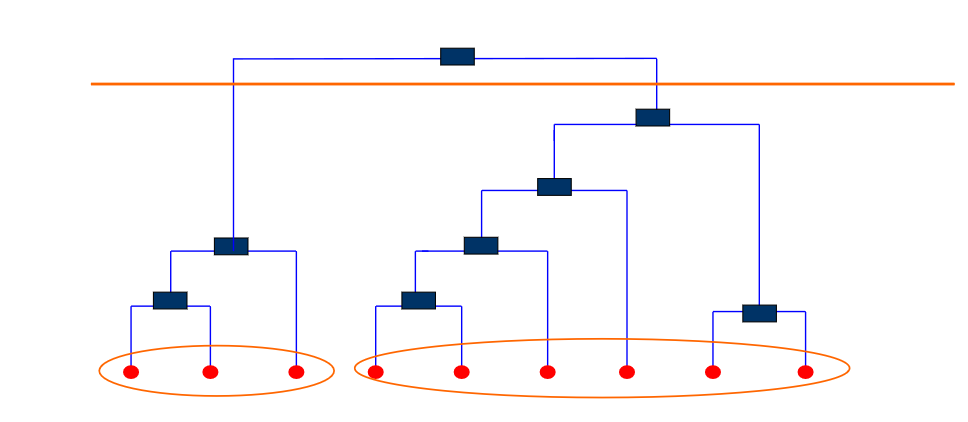
\includegraphics[width=0.8\textwidth]{dendogram.png}
                \caption{Dendogram}
                \label{fig:dendogram}
            \end{figure}

            A clustering of the data objects is obtained by cutting the dendrogram
            at the desired level, then each connected component forms a cluster
        \end{itemize}
    \end{answered}

    \item List, then define all possible methods of merging the clusters that depend on the distance measures.
    \begin{answered}
        \begin{description}
            \item[Single-link] The distance between two clusters is represented by
                               the distance of the \textcolor{Maroon}{\textbf{closest pair of data objects}}
                               belonging to different clusters.
            \item[Complete-link] The distance between two clusters is represented by
                                 the distance of the \textcolor{Maroon}{\textbf{farthest pair of data objects}}
                                 belonging to different clusters.
            \item[Average-link] The distance between two clusters is represented by
                                the average distance of \textcolor{Maroon}{\textbf{all pairs of data objects}}
                                belonging to different clusters.
            \item[Centroid distance] The distance between two clusters is represented by
                                     \textcolor{Maroon}{\textbf{the means of the clusters}}.
        \end{description}
    \end{answered}

    \item What are the advantages and disadvantages of hierarchical clustering?
    \begin{answered}
        \textbf{Advantages}
        \begin{itemize}
            \item Hierarchical clustering outputs a hierarchy, i.e., a
                structure that is more informative than the unstructured
                set of flat clusters returned by k-means. Therefore, it is
                easier to decide on the number of clusters by looking at the dendrograms
            \item Easy to implement
        \end{itemize}
        \textbf{Disadvantages}
        \begin{itemize}
            \item It is not possible to undo the previous step: once the
                instances have been assigned to a cluster, they can no
                longer be moved around.
            \item Time complexity: not suitable for large datasets
            \item Initial seeds have a strong impact on the final results
            \item The order of the data has an impact on the final results
            \item Very sensitive to outliers
        \end{itemize}
    \end{answered}

\end{QandA}

\section*{L17 Recommender Systems \textemdash{} Tue Mar 10}
\begin{QandA}

    \item Define the recommendation systems, why use Recommender Systems?
    \begin{answered}
        Recommendation systems are software agents that elicit the interests
        and preferences of individual consumers and make recommendations accordingly.
        They have the potential to support and improve the quality of the decisions
        consumers make while searching for and selecting products online.

        \textbf{Value for the customer}
        \begin{itemize}
            \item Find things that are interesting
            \item Narrow down the set of choices
            \item Help to explore the space of options
            \item Discover new things
            \item Entertainment
        \end{itemize}
        \textbf{Value for the provider}
        \begin{itemize}
            \item Additional and probably unique personalized service for the customer
            \item Increase trust and customer loyalty
            \item Increase sales, click through rates, conversion etc.
            \item Opportunities for promotion, persuasion
            \item Obtain more knowledge about customers
        \end{itemize}
    \end{answered}

    \item What types of recommendation systems, list them, then draw
          diagrams show the working mechanism of each?
    \begin{answered}
        \begin{enumerate}
            \item Content-based recommenders \textemdash{} Characteristic information
            \item Collaborative filtering recommenders \textemdash{} User-item interactions
        \end{enumerate}
        \begin{figure}[h!]
            \centering
            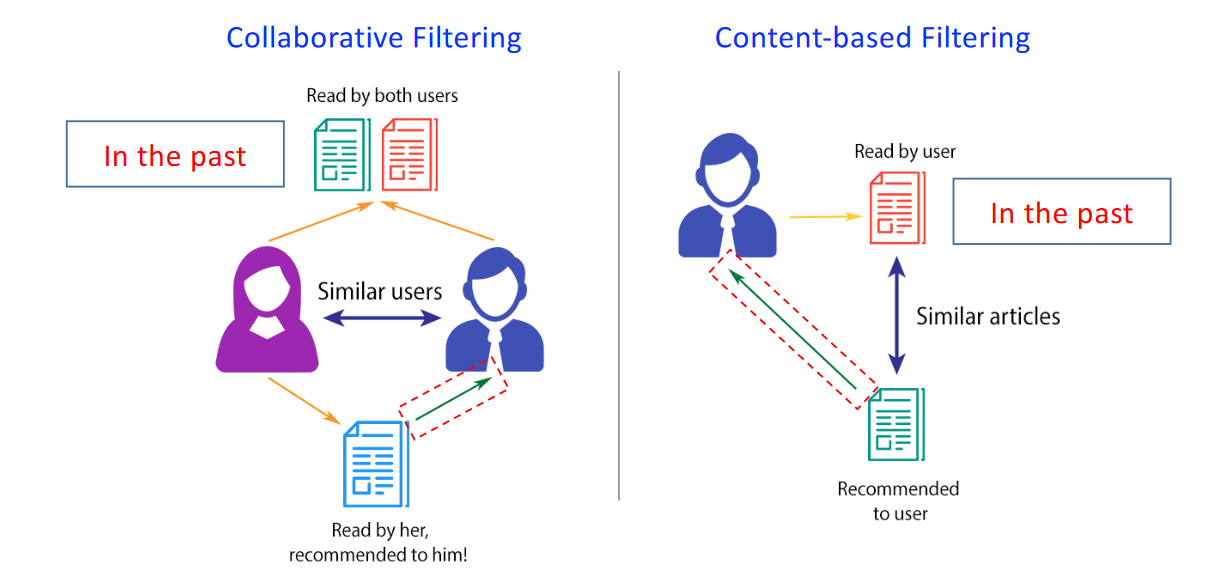
\includegraphics[width=0.8\textwidth]{recommenders.png}
            \caption{Recommender Types}
            \label{fig:recommenders}
        \end{figure}

    \end{answered}

    \item List advantages and disadvantages of both collaborative
          filtering and content-based recommenders.
    \begin{answered}
        \begin{itemize}
            \item \textbf{Collaborative filtering recommenders}

            \textbf{Advantages}
                \begin{itemize}
                    \item Doesn't require any knowledge about the products themselves
                \end{itemize}

            \textbf{Disadvantages}
                \begin{itemize}
                    \item Can't recommend products if you don't have user reviews
                    \item Difficult to make good recommendations for brand-new users
                    \item Tends to favor popular products with lots of reviews
                \end{itemize}

            \item \textbf{Content-based recommenders}

            \textbf{Advantages}
                \begin{itemize}
                    \item Works even when a product has no user reviews
                \end{itemize}

            \textbf{Disadvantages}
                \begin{itemize}
                    \item Needs descriptive data for every product that you want to recommend
                    \item Difficult to implement for many kinds of large product databases
                \end{itemize}
        \end{itemize}
    \end{answered}

    \item How to fill rates of users who have not rated any movies?
    \begin{answered}
        Perform \textit{Mean Normalization}, \textcolor{Maroon}{?? then assign 0 to each non-ranked movie.??}
        \begin{figure}[h!]
            \centering
            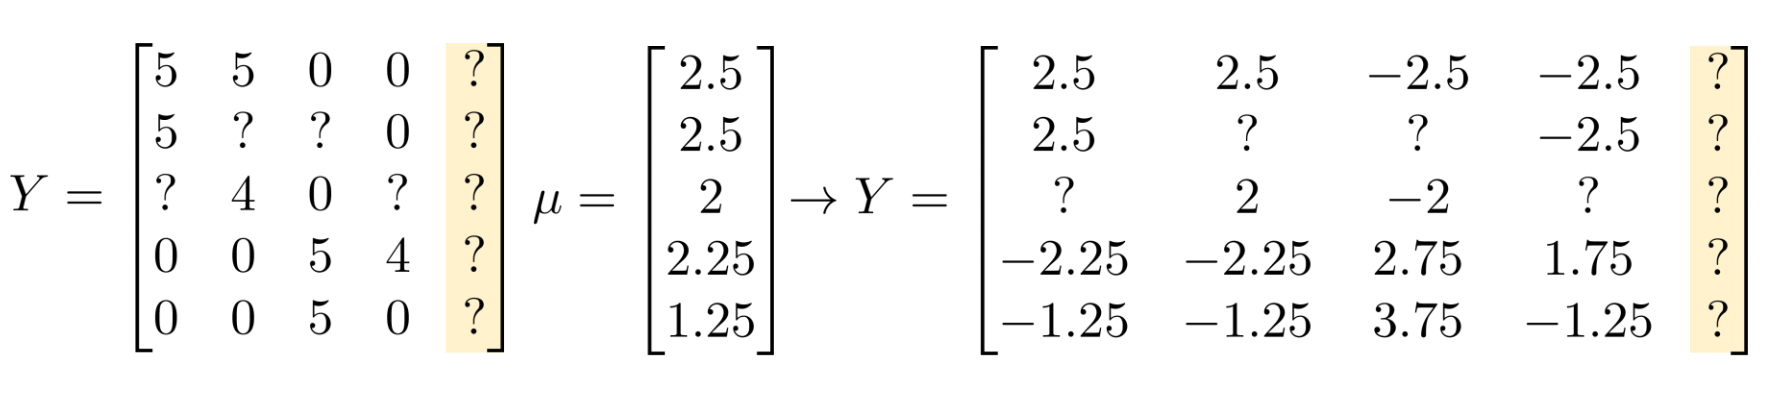
\includegraphics[width=0.8\textwidth]{mean_normalization.png}
            \caption{Mean Normalization}
            \label{fig:normalization}
        \end{figure}

    \end{answered}

\end{QandA}

\section*{L18 Large Scale and Online Learning  \textemdash{} Thu Mar 12}
\begin{QandA}
    \color{red}
    \item Supervised Learning, Semi-Supervised, and Unsupervised Learning
          for what kinds of applications can be used?
          What is the difference between them in terms of input and output samples?
    \color{black}
    \begin{answered}
    \end{answered}


    \item What are the differences between Gradient Descent types: Batch, Stochastic, and Mini batch?
          \textcolor{red}{Which one is the faster to converge? }
    \begin{answered}
        \begin{enumerate}
            \item Batch Gradient Descent: Uses all $m$ examples in each iteration
            \item Stochastic Gradient Descent: Uses 1 example in each iteration
            \item Mini-batch Gradient Descent: Uses $b$ examples in each iteration
        \end{enumerate}

    \end{answered}

    \item What are the hardware-based solutions can be used to machine learning for big data?
    \begin{answered}
        \begin{description}
            \item[Map-Reduce] Distributing data sets (e.g., training set) across networked computing devices (PCs)
            \item[Multi-core Machines] Distributing data sets (e.g., training set) across chip-scale computing devices
        \end{description}
    \end{answered}

    \item What are the platforms for online machine learning algorithms?
    \begin{answered}
        \begin{itemize}
            \item Hydrosphere.io
            \item Prediction.io
            \item Azure Machine Learning
            \item Amazon Machine Learning
            \item Google Prediction
            \item BigML
            \item DataRobot
        \end{itemize}
    \end{answered}

\end{QandA}

\section*{L19 Ensemble Learning \textemdash{} Thu Mar 19}
\begin{QandA}
    \item Define  \textit{ensemble learning}, illustrate the key motivation of ensemble learning, then draw the general idea diagram of the ensemble learning
    \begin{answered}
        \begin{description}
            \item[Ensemble learning] is a machine-learning paradigm where multiple learners are 
            trained to solve the same problem. In contrast to ordinary machine-learning approaches 
            that try to learn one hypothesis from training data, ensemble methods try to construct 
            a set of hypotheses and combine them into one.
        \end{description}
        The key motivation is to reduce the error rate. The expectation is that it will become much more unlikely 
        that the ensemble will misclassify an example.
    \end{answered}

    \item List the ensemble methods that minimize variance and bias.
    \begin{answered}
        \textbf{Minimize Variance}
        \begin{itemize}
            \item Bagging
            \item Random Forests
        \end{itemize}

        \textbf{Minimize Bias}
        \begin{itemize}
            \item Functional Gradient Descent
            \item Boosting
            \item Ensemble Selection
        \end{itemize}
    \end{answered}

    \item What are the different methods for changing training data? List them, then illustrate 
          the working mechanism of each method, support your working mechanisms with illustration diagrams.
    \begin{answered}
        \begin{description}
            \item[Bagging:] Resample training data (\textbf{see figure \ref{fig:bagging}})
            \item[Boosting:] Reweight training data (\textbf{see figure \ref{fig:boosting}})
        \end{description}
        \begin{figure}[h!]
            \centering
            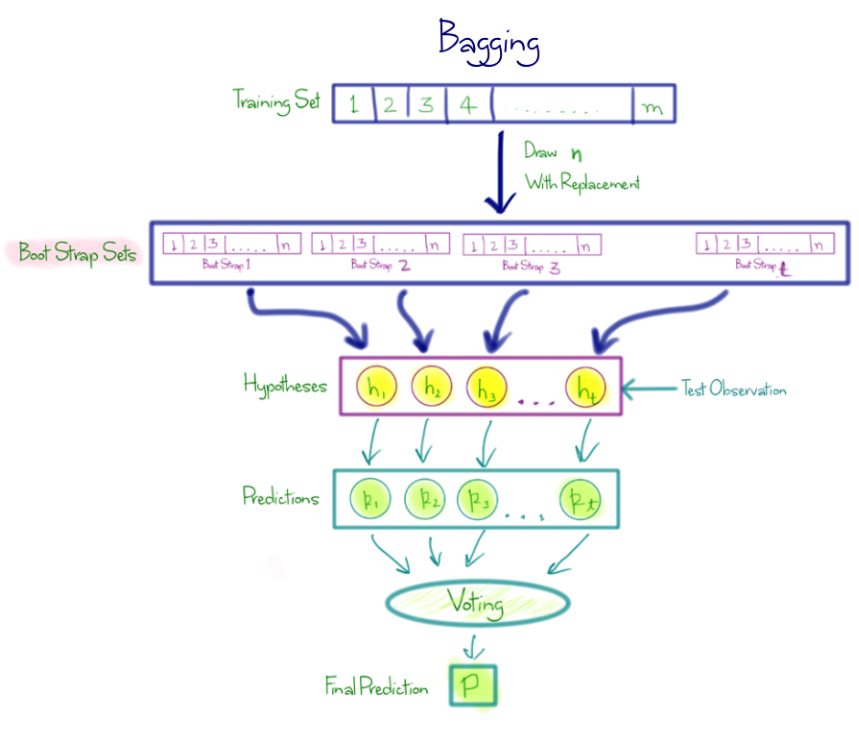
\includegraphics[width=0.5\textwidth]{bagging.png}
            \caption{Bagging}
            \label{fig:bagging}
        \end{figure}

        \begin{figure}[h!]
            \centering
            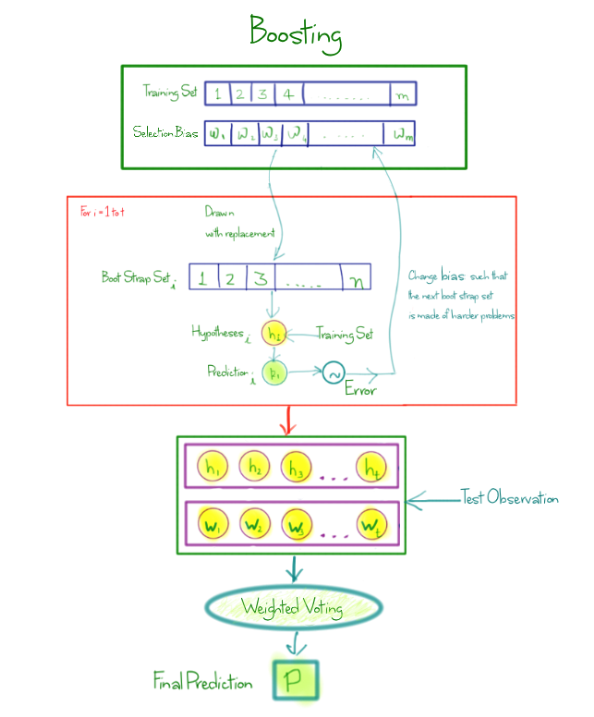
\includegraphics[width=0.5\textwidth]{boosting.png}
            \caption{Boosting}
            \label{fig:boosting}
        \end{figure}
    \end{answered}

    \item Can a set of weak learners create a single strong learner?
    \begin{answered}
        Yes.  You can construct a strong classifier by weighted voting of the 
        weak classifiers.

        The idea is that:
        \begin{itemize}
            \item Better weak classifier gets a larger weight
            \item Weak classifiers are added iteratively, which provides
                  increased accuracy through minimization of the cost function.
        \end{itemize}
    \end{answered}

    \item What are the main features of the Random Forest method?
    \begin{answered}
        \begin{itemize}
            \item Random Forest is an ensemble of Decision Trees.
            \item They are known to run efficiently on large datasets.
            \item Can take care of large number of features.
        \end{itemize}
\end{answered}

\end{QandA}

\section*{L20 k-Nearest Neighbors (kNNs) \textemdash{} Tue Mar 24}
\begin{QandA}
    \item What are the Idea, algorithm, and types of the Instance-Based Learning?
    \begin{answered}
        \subsubsection*{Idea}
        \begin{itemize}
            \item Similar examples have similar labels.
            \item Classify new examples like similar training examples.
        \end{itemize}
        \subsubsection*{Algorithm}
        \begin{itemize}
            \item Given some new example $x$ for which we need to predict its class $y$
            \item Find most similar training examples
            \item Classify $x$ “like” these most similar examples
        \end{itemize}
        \subsubsection*{Types}
        \begin{description}
            \item[Rote-learner] Memorizes entire training data and performs classification 
                                only if attributes of the record match one of the training examples exactly.
            \item[Nearest Neighbor] Uses $k$ \textit{closest} points (nearest neighbors) for performing classification.
        \end{description}
    \end{answered}

    \item List the k-Nearest Neighbors (k-NNs) Main Steps.
    \begin{answered}
        \begin{enumerate}
            \item For a given instance $T$, get the top $k$ dataset instances that are "nearest" to $T$ (select a reasonable distance measure).
            \item Inspect the category of these $k$ instances, choose the category $C$ that represent the most instances.
            \item Conclude that $T$ belongs to category $C$.
        \end{enumerate}
    \end{answered}

    \item What are the three require things to implement the k-NNs?
    \begin{answered}
        \begin{enumerate}
            \item \textbf{Feature Space} (Training Data)
            \item \textbf{Distance metric} (to compute distance between instances)
            \item The \textbf{value of $\mathbf{k}$} (the number of nearest neighbors to retrieve from which to get majority class)
        \end{enumerate}
    \end{answered}

    \item How to classify an unknown instance (sample) using the k-NNs?
    \begin{answered}
        \begin{enumerate}
            \item Compute distance to other training instances
            \item Identify $k$ nearest neighbors (k-NNs)
            \item Use class labels of nearest neighbors to determine the class label of the unknown instance
        \end{enumerate}
    \end{answered}

    \item What are the two common distance metrics used for k-NNs?
    \begin{answered}
        \begin{description}
            \item[Euclidean Distance (Continuous distribution):] the square root of the sum of the squared differences between a new point (x) and an existing point (y)
            \item[Manhattan Distance:] the distance between real vectors using the sum of their absolute difference
        \end{description}
    \end{answered}

    \item List Advantages and Disadvantages of k-NNs.
    \begin{answered}
        \subsubsection*{Advantages}
            \begin{itemize}
                \item Simple technique that is easily implemented
                \item Building model is inexpensive 
                \item Extremely flexible classification scheme \textemdash{} does not involve preprocessing
                \item Well suited for
                    \begin{itemize}
                        \item Multi-modal classes (classes of multiple forms)
                        \item Records with multiple class labels
                    \end{itemize}
                \item Can sometimes be the best method
            \end{itemize}
        \subsubsection*{Disadvantages}
            \begin{itemize}
                \item Classifying unknown records are relatively expensive
                    \begin{itemize}
                        \item Requires distance computation of k-nearest neighbors
                        \item Computationally intensive, especially when the size of the training set grows
                    \end{itemize}
                \item Accuracy can be severely degraded by the presence of noisy or irrelevant features
                \item Nearest-neighbor classification expects class conditional probability to be locally constant
            \end{itemize}
    \end{answered}
\end{QandA}

\section*{L21 Principle Components Analysis (PCA) \textemdash{} Thu Mar 26}
\begin{QandA}
    \item Define principle components analysis (PCA), then list the 3 main fields could be used to and 3 application examples.
    \begin{answered}
        \subsubsection*{Principle Components Analysis (PCA)}
        \begin{itemize}
            \item A technique used to reduce the dimensionality of the data set to 2D or 3D.
            \item PCA allows us to compute a linear transformation that maps data from a high dimensional space to a lower dimensional sub-space.
            \item The goal of PCA is to reduce the dimensionality of the data while retaining as much information as possible in the original dataset.
        \end{itemize}
        Can be used to:
        \begin{enumerate}
            \item Reduce number of dimensions in data
            \item Find patterns in high-dimensional data
            \item Visualize data of high dimensionality
        \end{enumerate}
        Example applications:
        \begin{enumerate}
            \item Face recognition
            \item Image compression
            \item Gene expression analysis
        \end{enumerate}
    \end{answered}

    \item What do we mean by the variance and covariance? List the differences between the variance and covariance.
    \begin{answered}
        \begin{description}
            \item[Variance and Covariance:] Measure of the \textit{spread} of a set of points around their center of mass (mean)
            \item[Variance:] Measure of the deviation from the \textit{mean} for points in \textit{one dimension}
            \item[Covariance:] Measure of how much each of the dimensions vary from the mean with \textit{respect to each other}
            \begin{itemize}
                \item Covariance is measured between two dimensions
                \item Covariance sees if there is a relation between two dimensions
                \item Covariance between one dimension is the variance
            \end{itemize} 
        \end{description}
    \end{answered}

    \item Illustrate the main tasks of the PCA Process \textemdash{} step 1.
    \begin{answered}
        \begin{itemize}
            \item Subtract the \textit{mean} from each of the data dimensions.
            \item All the $x$ values have $x$ subtracted and $y$ values have $y$ subtracted from them.
            \item This produces a dataset whose mean is zero.
            \item Subtracting the mean makes variance and covariance calculation easier by simplifying their equations.
            \item The variance and co-variance values are not affected by the mean value.
        \end{itemize}
    \end{answered}

    \item How we could derive new datasets through the PCA Process \textemdash{} step 5?
    \begin{answered}
        \begin{enumerate}
            \item Final Data = \textit{Row Feature Vector} $\times$ \textit{Row Zero Mean Data}
            
            \item \textit{Row Feature Vector} is the matrix with the eigenvectors in the 
                  columns transposed so that the eigenvectors are now in the rows, 
                  with the most significant eigenvector at the top.

            \item \textit{Row Zero Mean Data} is the mean-adjusted data transposed; 
                  i.e., the data items are in each column, with each row holding 
                  a separate dimension.
        \end{enumerate}
    \end{answered}

\end{QandA}

\section*{L22 Recurrent Neural Networks \textemdash{} Tue Apr 7}
\begin{QandA}
    \item Define RNNs.
    \begin{answered}
        Neural nets that allow previous outputs to be used as inputs while having hidden states.
    \end{answered}

    \item Are RNNs Supervised or Unsupervised Learning?
    \begin{answered}
        Supervised: used for time series analysis.
    \end{answered}

    \item What is the major difference between RNNs and FNNs? illustrate that.
    \begin{answered}
        In feed-forward neural networks, the connections between nodes do not form a cycle.  However,
        in recurrent neural networks, the connections between nodes form cyclic paths.
    \end{answered}

    \item List types AND architectures of RNNs, then draw the architecture of traditional RNNs.
    \begin{answered}
        \begin{enumerate}
            \item One-to one
            \item One-to-many
            \item Many-to-one
            \item Many-to-many
        \end{enumerate}
        \begin{figure}[h!]
            \centering
            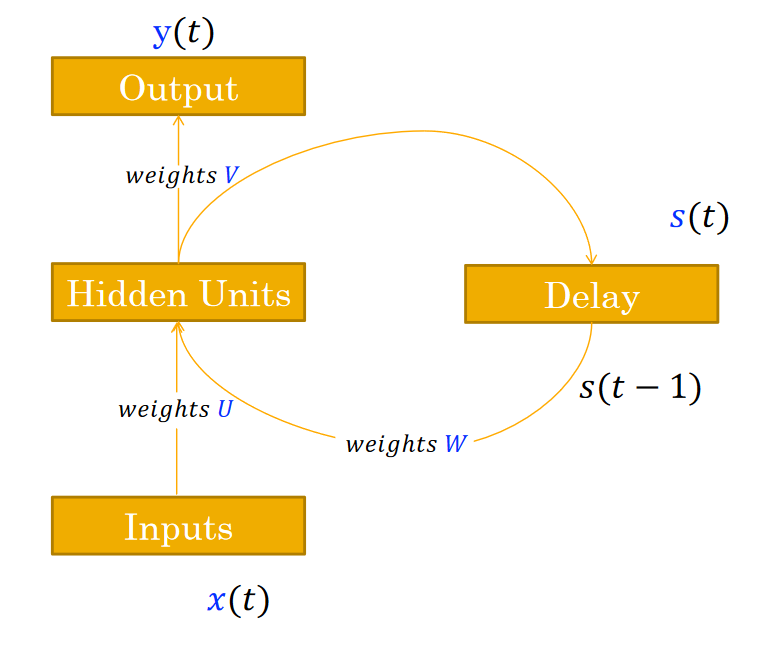
\includegraphics[width=0.5\textwidth]{rnn.png}
            \caption{Architecture of a traditional RNN}
            \label{fig:rnn}
        \end{figure}

    \end{answered}

    \item List, \textcolor{red}{then illustrate the three main training approaches of RNNs.}
    \begin{answered}
        \begin{description}
            \item[Back-propagation through-time:] Unfolding RNNs in time and using the extended version of back-propagation.
            \item[Extended Kalman Filtering (EKF):] A set of mathematical equations that provides efficient computational means to estimate the state of a process, in a way that minimizes the mean of squared error (cost function) on a linear system.
            \item[Real-Time Recurrent Learning (RTRL):] Computing the error gradient and update weights for each time step.
        \end{description}
        \begin{figure}[h!]
            \centering
            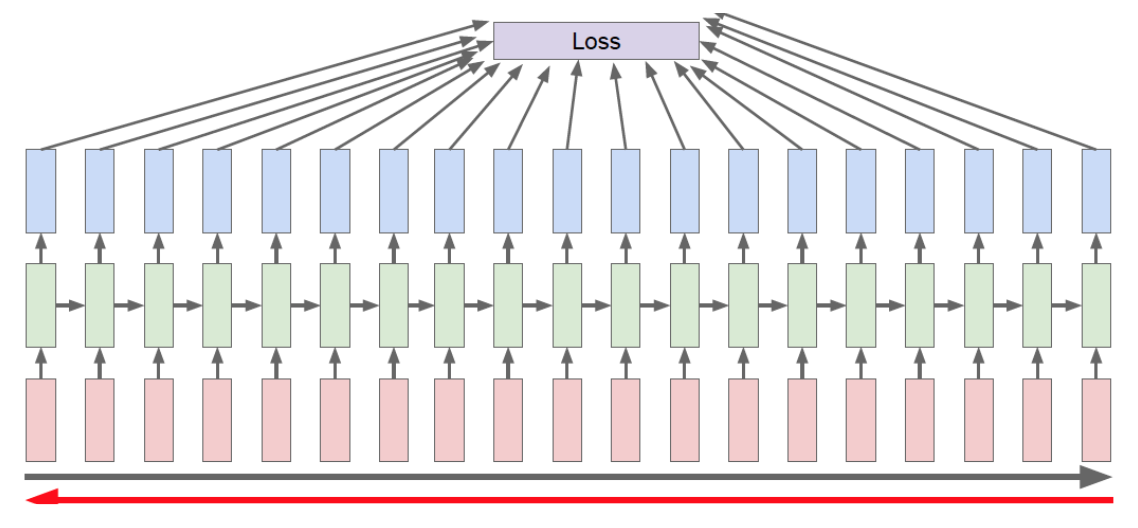
\includegraphics[width=0.5\textwidth]{back_prop_time.png}
            \caption{Back-propagation through time}
            \label{fig:backprop}
        \end{figure}
    \end{answered}

    \item What are the pros and cons of the typical RNNs architecture?
    \begin{answered}
        \subsubsection*{Advantages}
        \begin{enumerate}
            \item Possibility of processing input of any length
            \item Model size $s$ not increasing with size of input
            \item Computation considers historical information
            \item Weights are shared across time
        \end{enumerate}
        \subsubsection*{Disadvantages}
        \begin{enumerate}
            \item Computation being slow
            \item Difficulty of accessing information from a long time ago
            \item Cannot consider any future input for the current state
        \end{enumerate}
    \end{answered}

\end{QandA}

\section*{L23 Reinforcement Learning \textemdash{} Thu Apr 9}
\begin{QandA}
    \item List the four main machine learning types.
    \begin{answered}
    \end{answered}

    \item Define the reinforcement learning with a diagram, then compare between the
          reinforcement learning and supervised learning.
    \begin{answered}
    \end{answered}

    \item Draw the generic learning model to learn from data. Then define the main operations of
          it through indicating each operation (i.e. Sensor Data, Feature Extraction, etc.) and
          related steps.
    \begin{answered}
    \end{answered}

    \item What are the key features and elements of the reinforcement learning?
    \begin{answered}
    \end{answered}

    \item List the 3 types of reinforcement learning.
    \begin{answered}
    \end{answered}

    \item What makes reinforcement learning different from other machine learning paradigms?
    \begin{answered}
    \end{answered}

\end{QandA}

\section*{L24 Autoencoders \textemdash{} Tue Apr 14}
\begin{QandA}
    \item What are autoencoders? List the general types of autoencoders based on size of hidden layer?
    \begin{answered}
    \end{answered}

    \item What are the main differences between PCA and autoencoders?
    \begin{answered}
    \end{answered}

    \item List the key elements AND components of autoencoders? Then illustrate the components.
    \begin{answered}
    \end{answered}

    \item List, then explain the 3 main properties AND 4 hyperparameters of autoencoders.
    \begin{answered}
    \end{answered}

    \item List the 8 types AND 5 applications of autoencoders.
    \begin{answered}
    \end{answered}

\end{QandA}

\section*{L25 Bayesian Networks \textemdash{} Thu Apr 16}
\begin{QandA}
    \item What are Bayesian networks (BNs)? List BN components and importance.
    \begin{answered}
    \end{answered}

    \item List types of probabilistic relationships, then provide 7 real-world Bayesian network applications.
    \begin{answered}
    \end{answered}

    \item Define hidden Markov model (HMM), then list and illustrate components of HMM.
    \begin{answered}
    \end{answered}

    \item List, with illustration, the 4 main inference algorithms of Hidden Markov Model.
    \begin{answered}
    \end{answered}

    \item What are advantages and disadvantages of Hidden Markov Model?
    \begin{answered}
    \end{answered}

\end{QandA}

\end{document}
